\chapter{Resultados}
	
	\section{Diseño del sistema desalinizador}
		
		Tras varias propuestas se llegó a un diseño modular vertical. En la~\cref{fig:WaterModule} se puede observar el primer módulo llamado ``Módulo de reaprovechamiento térmico y bombeo'' el cual se diseñó para aprovechar el calor del vapor generado tras pasar por el ``Módulo de concentración solar'' el cual se integra a un seguidor solar para calentar el agua indirectamente por medio de la lente de Fresnel.
		
		
		\begin{figure}[H]
			\centering
			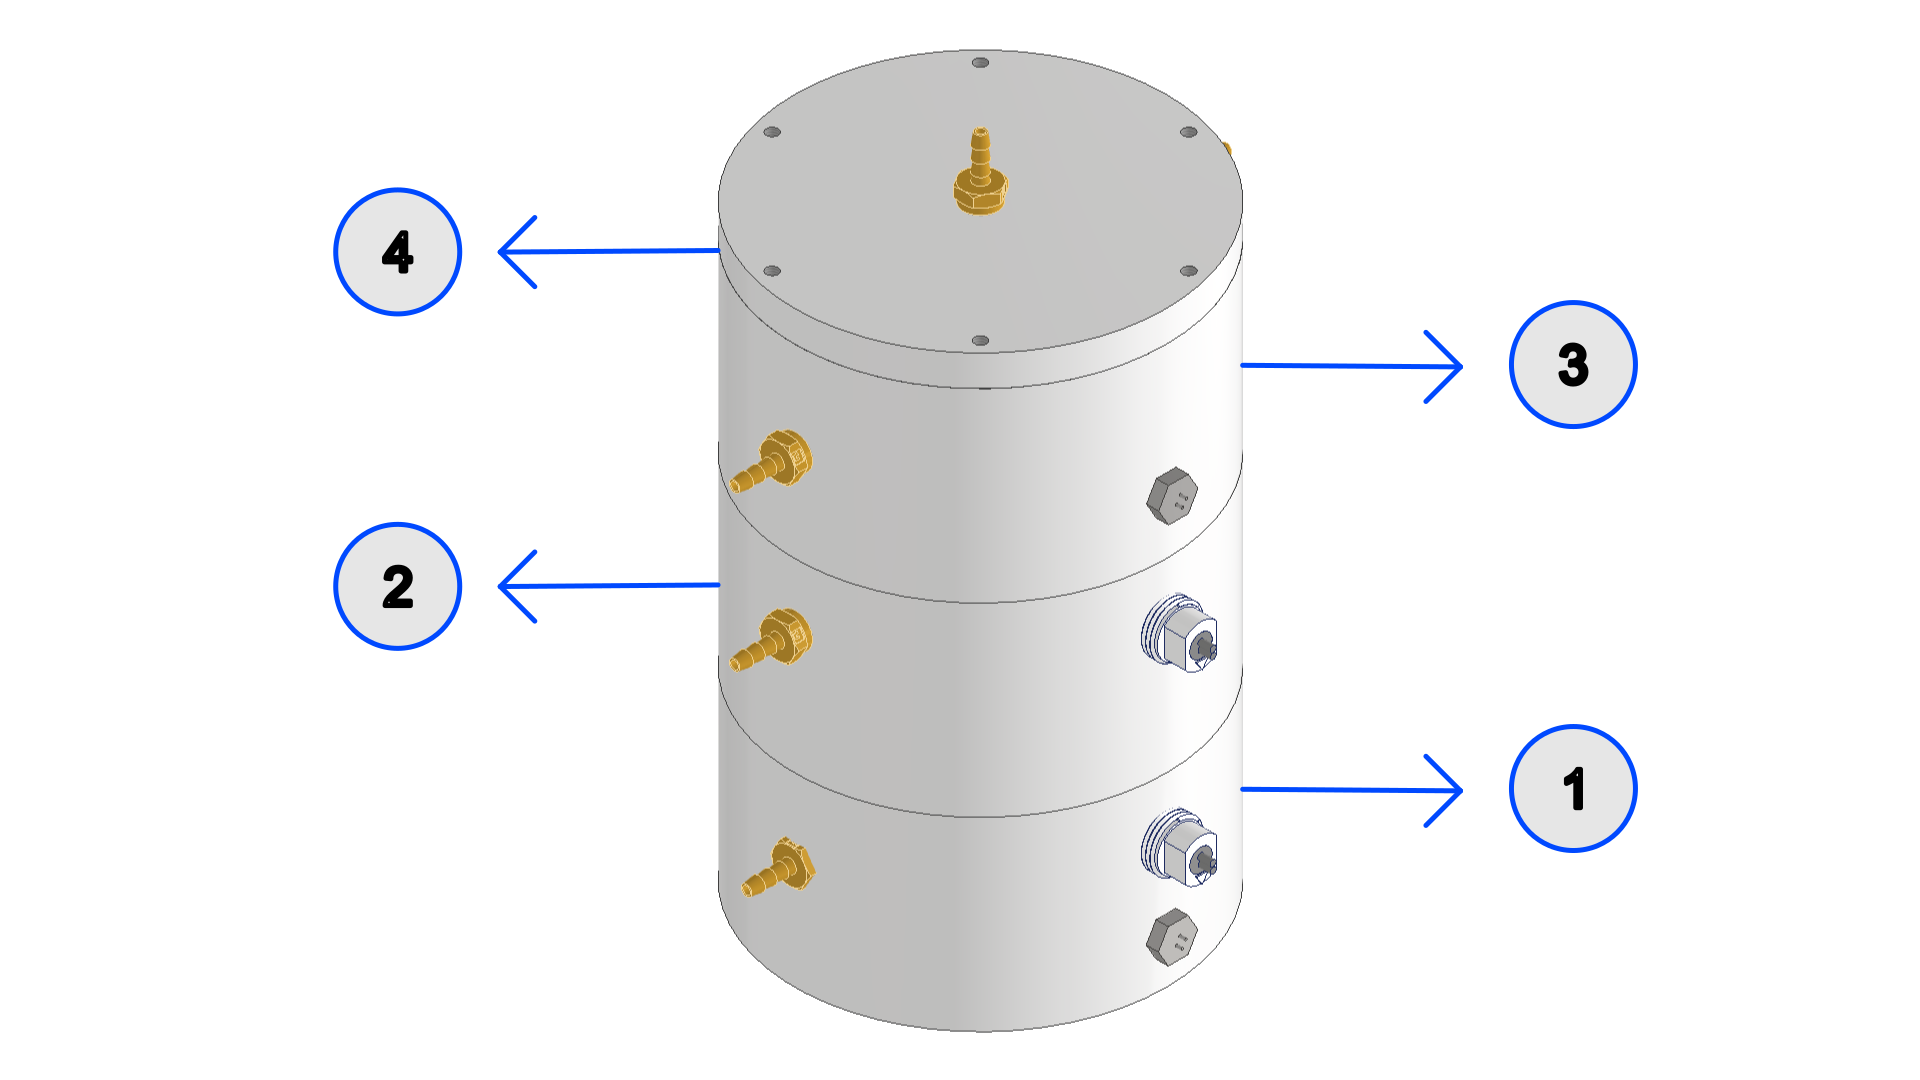
\includegraphics[
				width=\linewidth,
				height=70mm,
				keepaspectratio
			]{Resultados/Sistema/WaterModule.png}
			\caption{Propuesta del sistema desalinizador. Módulo de reaprovechamiento térmico y bombeo.}
			\label{fig:WaterModule}
		\end{figure}
		
		\begin{enumerate}
			\item Contenedor de agua de mar
			\item Contenedor de agua destilada
			\item Receptor para vaporización
			\item Tapa
		\end{enumerate}
		
		En las siguientes secciones se detallarán los elementos que componen a este sistema y las funciones que desempeñan.
	
		\subsection{Contenedor de agua de mar}
			
			Su función básica es contener el agua a desalinizar y servir al mismo tiempo como fuente de frío para la condensación del vapor.
			
			El contenedor de agua de mar consta de 2 entradas y 1 salida.
			\begin{itemize}[columns=2]
				\item Entrada de agua de mar
				\item Entrada del excedente de agua caliente a evaporar
				\item Salida hacia el Módulo de concentración solar
			\end{itemize}
			
			En este módulo se monitorea la temperatura y nivel del agua.
		
		\subsection{Contenedor de agua destilada}
			
			Su función básica es promover la condensación del vapor y favorecer el aumento de la temperatura del agua de entrada usando un intercambiador de calor entre la misma cámara y el contenedor de agua de mar.
			
			Este submódulo consta de 1 entrada y 2 salidas.
			
			\begin{itemize}[columns=2]
				\item Entrada de vapor caliente \columnbreak
				\item Salida para regular la presión entre cámaras
				\item Salida de agua destilada
			\end{itemize}
		
						
		\subsection{Cámara de evaporación}
			
			Su función básica es favorecer el proceso de evaporación aumentando el área superficial por unidad de volumen del agua de mar a su vez de mantener retroalimentación por gravedad hacia la cámara de agua de mar. Los elementos principales etiquetados en las \cref{fig:camara-evaporación-corte-1,fig:camara-evaporación-corte-2} se detallan a continuación: 1) Salida de agua altamente salina 2) Continuación del canal de alimentación hacia la cámara de concentración. 3) Salida de vapor hacia la cámara de condensado. D) Canales de desagüe para evitar la acumulación de agua salina.
		
			\begin{figure}[H]
				\centering
				\includegraphics[
					width=\linewidth,
					height=70mm,
					keepaspectratio
				]{Resultados/Cortes/camara-evaporación-corte-1.png}
				\caption{Cámara de evaporación. Corte 1}
				\label{fig:camara-evaporación-corte-1}
			\end{figure}
			
			\begin{figure}[H]
				\centering
				\includegraphics[
					width=\linewidth,
					height=70mm,
					keepaspectratio
				]{Resultados/Cortes/camara-evaporación-corte-2.png}
				\caption{Cámara de evaporación. Corte 2}
				\label{fig:camara-evaporación-corte-2}
			\end{figure}
			
		\subsection{Cámara de concentración}
			
			\subsubsection{Parte inferior}
				
				Su función básica es favorecer el proceso de evaporación aumentando el área superficial por unidad de volumen del agua de mar a su vez de mantener retroalimentación por gravedad hacia la cámara de agua de mar. Los elementos principales etiquetados en las \cref{fig:Arena-concentrador-corte-1,fig:Arena-concentrador-corte-2} se detallan a continuación: 1) Entrada del agua de mar. 2) Salida del agua de mar.
			
				\begin{figure}[H]
					\centering
					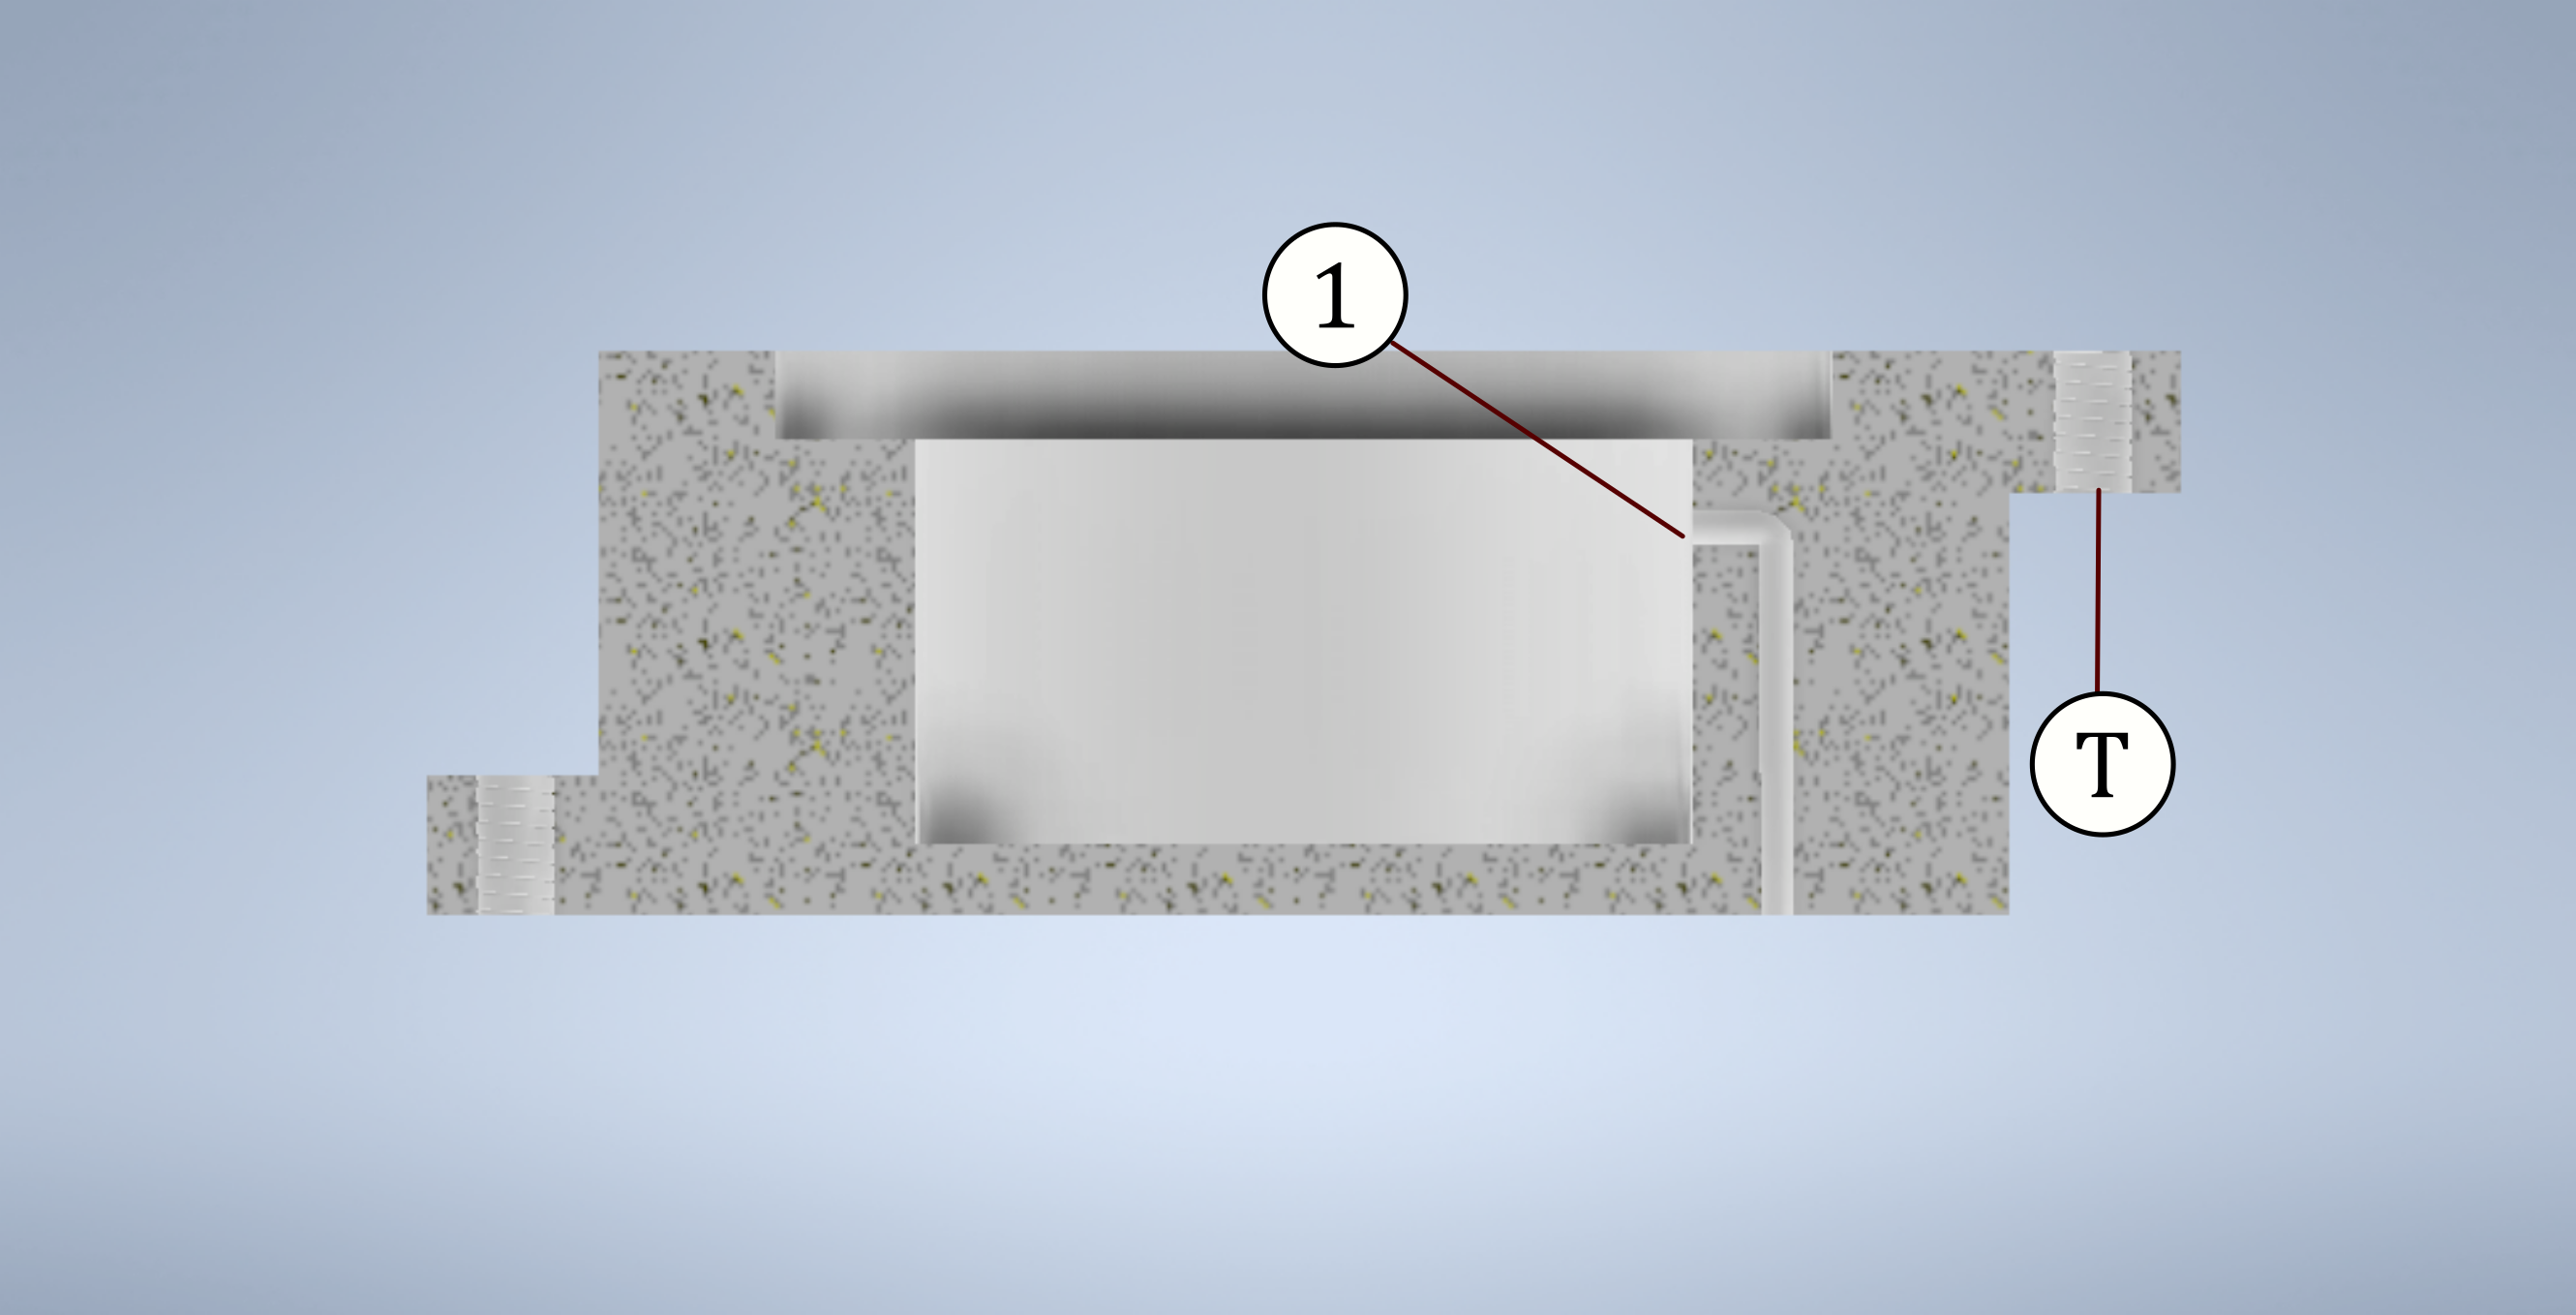
\includegraphics[
						width=\linewidth,
						height=70mm,
						keepaspectratio
					]{Resultados/Cortes/Arena-concentrador-corte-1.png}
					\caption{Cámara de concentración; parte inferior. Corte 1}
					\label{fig:Arena-concentrador-corte-1}
				\end{figure}
				
				\begin{figure}[H]
					\centering
					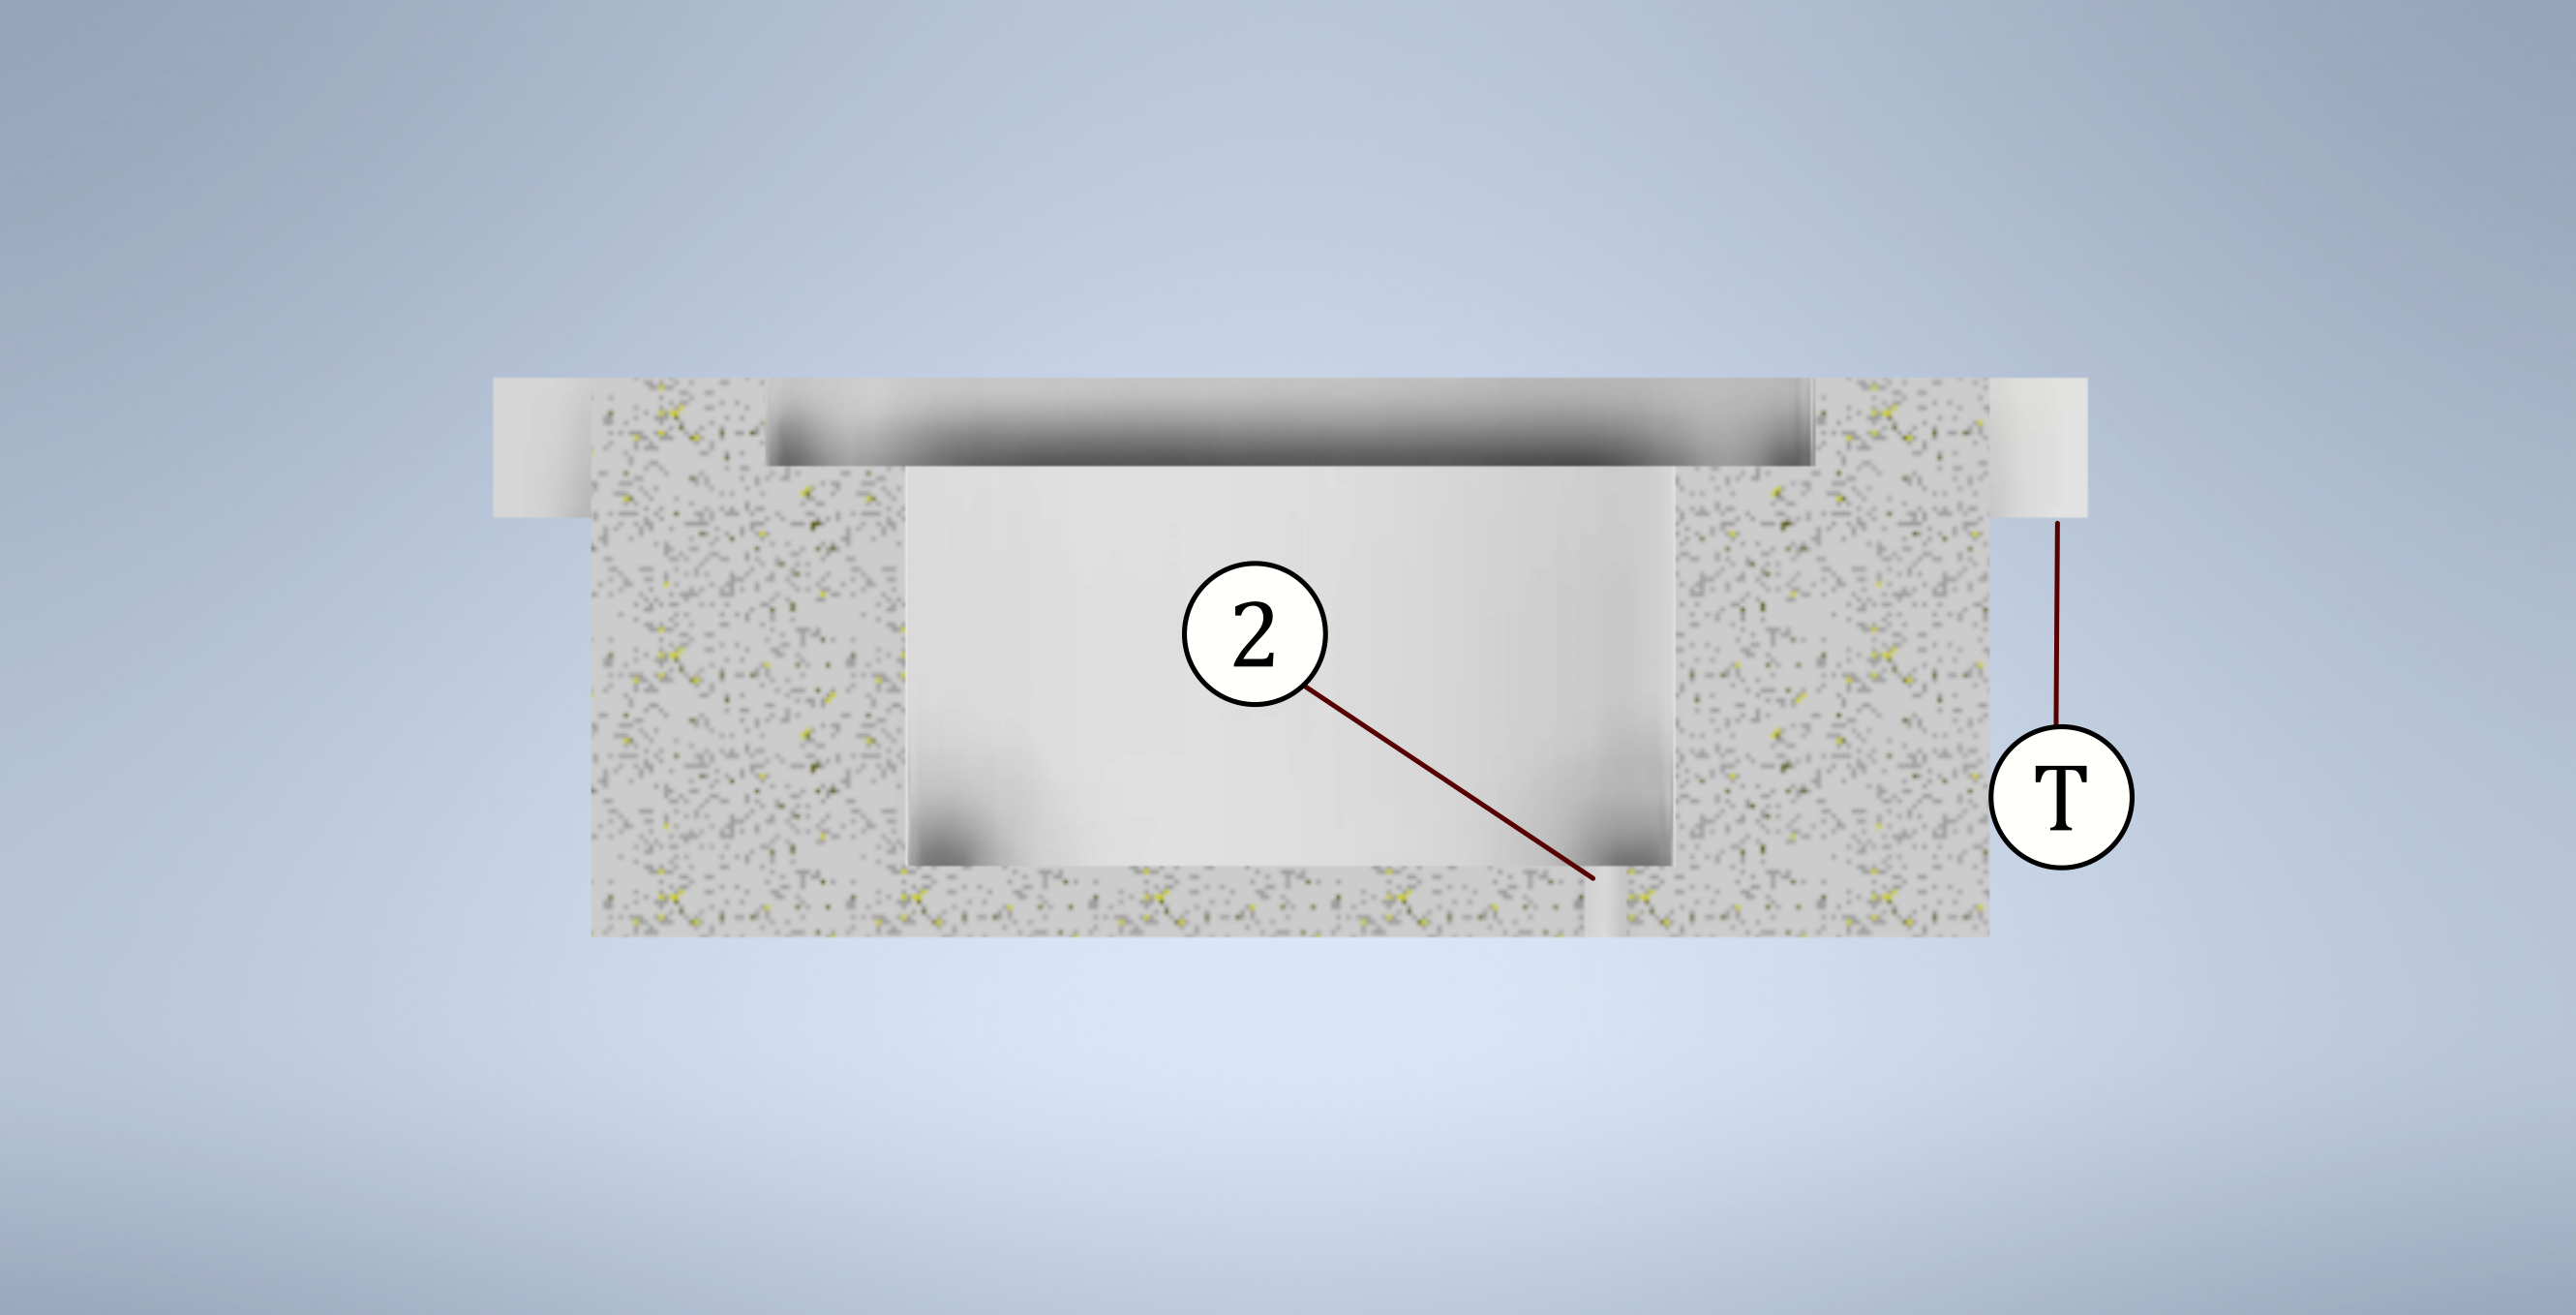
\includegraphics[
						width=\linewidth,
						height=70mm,
						keepaspectratio
					]{Resultados/Cortes/Arena-concentrador-corte-2.png}
					\caption{Cámara de concentración; parte inferior. Corte 2}
					\label{fig:Arena-concentrador-corte-2}
				\end{figure}
			
			\subsubsection{Parte superior}
				
				La parte superior de la cámara de concentración consta de la tapa que ayuda a la de sujeción del cristal de cuarzo y el recibidor solar. Estos se unen a la cámara inferior
			
			
%			\begin{figure}
%				\centering
%				\includegraphics[
%					width=\linewidth,
%					keepaspectratio
%				]{dsf}
%			\end{figure}
%		
%		Conductividad térmica
%		
%		Para conocer $\gls{cs}_{\text{agua}}$ de la \cref{table:Conductividad-térmica-agua-salada} se usa \eqref{equ:interpolación-lineal-simple} para obtener la conductividad estimada a los \qty{13}{\degreeCelsius} y a los \qty{94.7}{\degreeCelsius}.
%		
%		\begin{align*}
%			\gls{cs}_{13} &= \qty{0.586}{\watt\per\m\kelvin} + \dfrac{\qty{0.601}{\watt\per\m\kelvin} - \qty{0.586}{\watt\per\m\kelvin}}{\qty{20}{\degreeCelsius}-\qty{10}{\degreeCelsius}} \times (\qty{20}{\degreeCelsius} - \qty{13}{\degreeCelsius})\\
%			\gls{cs}_{13} &= \qty{0.591}{\watt\per\m\kelvin}\\
%			\gls{cs}_{94.7} &= \qty{0.670}{\watt\per\m\kelvin} + \dfrac{\qty{0.674}{\watt\per\m\kelvin} - \qty{0.670}{\watt\per\m\kelvin}}{\qty{100}{\degreeCelsius}-\qty{90}{\degreeCelsius}} \times (\qty{100}{\degreeCelsius} - \qty{94.7}{\degreeCelsius})\\
%			\gls{cs}_{94.7} &= \qty{0.672}{\watt\per\m\kelvin}
%		\end{align*}
%		
%		Una vez obtenidos sacamos el promedio incluyendo el resto del intervalo dándonos que:
%		\begin{equation*}
%			\gls{cs}_{\text{agua}} = \qty{0.638}{\watt\per\m\kelvin}
%		\end{equation*}